\documentclass{standalone}
\usepackage{ifthen}
\usepackage{physics}
\usepackage{tikz}
\usepackage{tikzlings-koalas}
\usetikzlibrary{calc}
\begin{document}
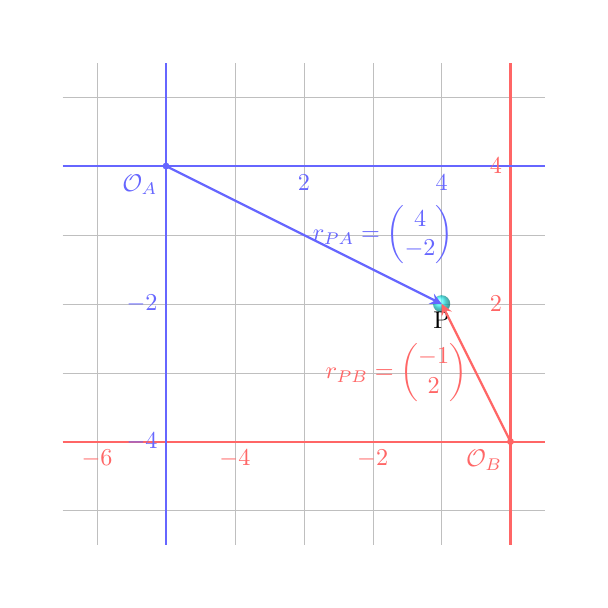
\begin{tikzpicture}[scale = 7/8, transform shape]
	\def\r{.05}
	\def\px{2}
	\def\py{0}
	\def\ax{-2}
	\def\ay{2}
	\def\bx{3}
	\def\by{-2}
	\def\TickSize{.01cm}
	\def\colA{blue!60!white}
	\def\colB{red!60!white}
	\coordinate (P) at (\px,\py);
	\coordinate (A) at (\ax,\ay);
	\coordinate (B) at (\bx,\by);
	\draw[white] (-4,-4) -- (4,4);
	\draw[step=1,gray!50!white,ultra thin] (-3.5,-3.5) grid (3.5,3.5);
	
%		\koala[body = black!60!white,xshift = \ax, yshift = \ay, scale = .4];
%		\koala[body = black!45!white,xshift = \bx, yshift = \by, scale = .4];
	\shade[ball color= cyan,opacity=0.7] (P) circle[radius=.125];
	
	\node[below] at (P) {P};
%		\node[below] at (A) {A};
	\fill[\colA] (A) circle ({\r});
%		\node[below] at (B) {B};
	\fill[\colB] (B) circle ({\r});
	
	
	\node[anchor = north east, color = \colB] at (B) {\(\mathcal{O}_B\)};
	\draw[\colB,thick] (-3.5,\by) -- (3.5,\by);
	\draw[\colB,thick] (\bx,-3.5) -- (\bx,3.5);
	
	\node[anchor = north east, color = \colA] at (A) {\(\mathcal{O}_A\)};
	\draw[\colA,thick] (-3.5,\ay) -- (3.5,\ay);
	\draw[\colA,thick] (\ax,-3.5) -- (\ax,3.5);
	
	\foreach \x in {-3,-2,...,3} {
		\pgfmathparse{Mod(\x - \bx,2)==0?1:0}
		\ifthenelse{\pgfmathresult = 0 \OR \x = \bx}{
		\node[anchor = north, color = \colB] at (\x,\by) { };
		}{
		\node[anchor = north, color = \colB] at (\x,\by) {\pgfmathparse{\x - \bx}\pgfmathprintnumber{\pgfmathresult}};
		}
	}

	\foreach \y in {-3,-2,...,3} {
		\pgfmathparse{Mod(\y - \by,2)==0?1:0}
		\ifthenelse{\pgfmathresult = 0 \OR \y = \by}{
			\node[anchor = east, color = \colB] at (\bx,\y) { };
		}{
			\node[anchor = east, color = \colB] at (\bx,\y) {\pgfmathparse{\y - \by}\pgfmathprintnumber{\pgfmathresult}};
		}
	}

	\foreach \x in {-3,-2,...,3} {
		\pgfmathparse{Mod(\x - \ax,2)==0?1:0}
		\ifthenelse{\pgfmathresult = 0 \OR \x = \ax}{
				\node[anchor = north, color = \colA] at (\x,\ay) { };
			}{
				\node[anchor = north, color = \colA] at (\x,\ay) {\pgfmathparse{\x - \ax}\pgfmathprintnumber{\pgfmathresult}};
			}
		}
		
		\foreach \y in {-3,-2,...,3} {
			\pgfmathparse{Mod(\y - \ay,2)==0?1:0}
			\ifthenelse{\pgfmathresult = 0 \OR \y = \ay}{
				\node[anchor = east, color = \colA] at (\ax,\y) { };
			}{
				\node[anchor = east, color = \colA] at (\ax,\y) {\pgfmathparse{\y - \ay}\pgfmathprintnumber{\pgfmathresult}};
			}
		}
		
		\draw[\colA,-stealth, thick] (A) -- (P) node[pos = .5, anchor = west]{\(r_{PA} = \mqty(\pgfmathparse{\px - \ax}\pgfmathprintnumber{\pgfmathresult}\\\pgfmathparse{\py - \ay}\pgfmathprintnumber{\pgfmathresult})\)};
		
		\draw[\colB,-stealth, thick] (B) -- (P) node[pos = .5, anchor = east]{\(r_{PB} = \mqty(\pgfmathparse{\px - \bx}\pgfmathprintnumber{\pgfmathresult}\\\pgfmathparse{\py - \by}\pgfmathprintnumber{\pgfmathresult})\)};
	\end{tikzpicture}
\end{document}
